\documentclass[11pt,a4paper]{article}
\usepackage[UTF8]{ctex}
\usepackage{geometry}
\usepackage{xcolor}
\usepackage{hyperref}
\usepackage{tikz}
\usetikzlibrary{positioning, shapes.geometric, arrows}

\geometry{margin=1in}

%=================================================
% 封面
%=================================================
\begin{document}

\begin{titlepage}
    \centering
    \vspace*{2cm}
    {\huge\textbf{深 \quad 圳 \quad 大 \quad 学}}\\[0.6cm]
    {\Large\textbf{Python 程序设计实验报告}}\\[2cm]

    \begin{flushleft}
    \large
    \textbf{课程名称:} Python 程序设计\\[0.3cm]
    \textbf{实验项目:} Alien Invasion 游戏设计实验\\[0.3cm]
    \textbf{指导老师:} 樊超\\[0.3cm]
    \textbf{学生姓名:} 刘辰\\[0.3cm]
    \textbf{学\hspace{0.8em}号:} 2024401003\\[0.3cm]
    \textbf{提交日期:} 2025 年 11 月 18 日
    \end{flushleft}

    \vfill
\end{titlepage}

%=================================================
% 摘要与正文
%=================================================

\begin{center}
\textbf{项目源码:}  
\href{https://github.com/santa3-1-1/Alien_invasion}{https://github.com/santa3-1-1/Alien\_invasion}
\end{center}

\section*{摘要}
本项目基于 Python + Pygame 开发 2D 射击游戏 \textbf{Alien Invasion},支持飞船移动、射击、外星舰队生成、关卡推进等核心机制。在课程基础要求之上,本人实现了用户系统、UI 菜单、道具、Boss 多阶段攻击、视频动画渲染、多用户数据管理等扩展内容,使项目达到完整课程设计级别。

本人主要负责:\textcolor{red}{用户管理、UI、状态机架构、Boss 动画渲染、舰队逻辑、道具系统、成绩保存等关键功能}。

\section*{1. 项目内容}
目标是实现一个结构清晰、可扩展的 2D 游戏。基础功能包括飞船控制、外星人移动、碰撞检测、计分与关卡管理。

为了增强游戏性,本人扩展了多项功能,其中部分模块难度远高于课程基础要求,例如视频帧渲染、状态机解耦和 UI 组件构建等,这些均体现了项目的工程化设计能力。

\subsection*{创新扩展功能}
\begin{itemize}
    \item \textcolor{red}{多用户注册/登录 + 成绩记录系统}
    \item \textcolor{red}{完整 UI 组件库(按钮、输入框、菜单界面)}
    \item \textcolor{red}{集中式状态机框架,管理开始/暂停/战斗/结束等状态}
    \item \textcolor{red}{Boss 视频动画渲染 + 多阶段攻击模式}
    \item \textcolor{red}{随机道具掉落、效果判定与 Buff 实现}
    \item \textcolor{red}{游戏逻辑优化:帧缓存、事件循环处理、碰撞高效检测}
\end{itemize}

\section*{2. 系统设计(模块结构图)}

\vspace{0.3cm}
\begin{center}
\textbf{—— 以下红色模块为重点创新部分 ——}
\end{center}

\begin{center}
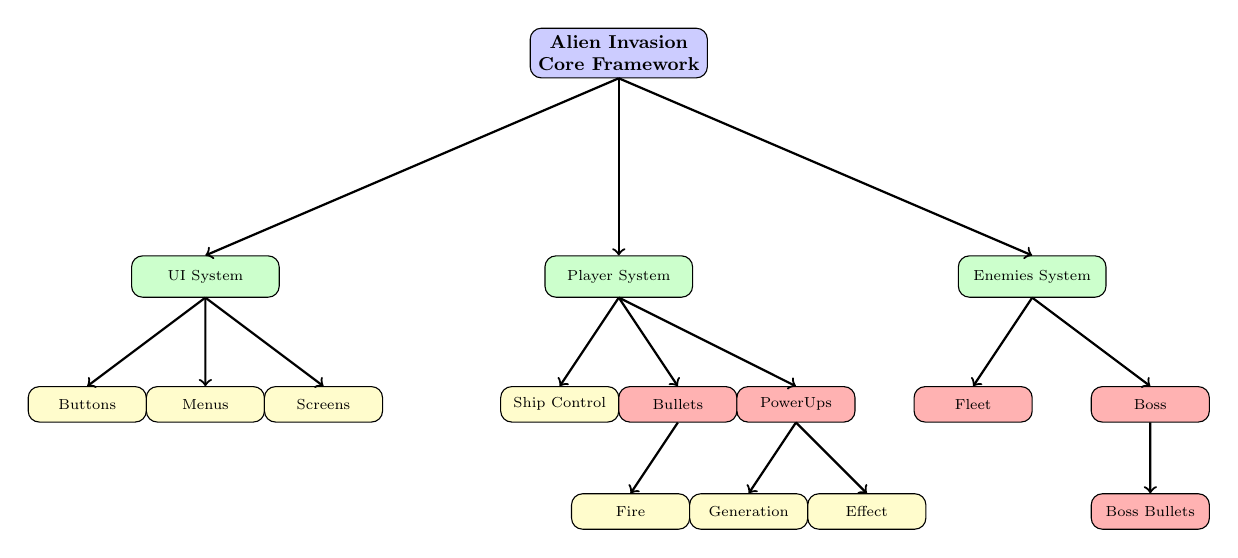
\begin{tikzpicture}[scale=0.75, transform shape,
    core/.style={rectangle, draw, rounded corners, minimum width=3cm, minimum height=0.8cm, align=center, fill=blue!20, font=\small\bfseries},
    module/.style={rectangle, draw, rounded corners, minimum width=2.5cm, minimum height=0.7cm, align=center, fill=green!20, font=\scriptsize},
    subsystem/.style={rectangle, draw, rounded corners, minimum width=2cm, minimum height=0.6cm, align=center, fill=yellow!20, font=\scriptsize},
    mypart/.style={rectangle, draw, rounded corners, minimum width=2cm, minimum height=0.6cm, align=center, fill=red!30, font=\scriptsize},
    arrow/.style={->, thick}
]

\node[core] (game) {Alien Invasion\\Core Framework};

\node[module, below=3cm of game, xshift=-7cm] (ui) {UI System};
\node[module, below=3cm of game] (player) {Player System};
\node[module, below=3cm of game, xshift=7cm] (enemies) {Enemies System};

\node[subsystem, below=1.5cm of ui, xshift=-2cm] (ui_buttons) {Buttons};
\node[subsystem, below=1.5cm of ui] (ui_menus) {Menus};
\node[subsystem, below=1.5cm of ui, xshift=2cm] (ui_screens) {Screens};

\node[subsystem, below=1.5cm of player, xshift=-1cm] (ship_control) {Ship Control};
\node[mypart, below=1.5cm of player, xshift=1cm] (bullets) {Bullets};
\node[mypart, below=1.5cm of player, xshift=3cm] (powerups) {PowerUps};

\node[subsystem, below=1.2cm of bullets, xshift=-0.8cm] (bullet_fire) {Fire};
\node[subsystem, below=1.2cm of powerups, xshift=-0.8cm] (pu_gen) {Generation};
\node[subsystem, below=1.2cm of powerups, xshift=1.2cm] (pu_effect) {Effect};

\node[mypart, below=1.5cm of enemies, xshift=-1cm] (fleet) {Fleet};
\node[mypart, below=1.5cm of enemies, xshift=2cm] (boss) {Boss};
\node[mypart, below=1.2cm of boss] (boss_bullets) {Boss Bullets};

\foreach \source/\dest in {
    game/ui, game/player, game/enemies,
    ui/ui_buttons, ui/ui_menus, ui/ui_screens,
    player/ship_control, player/bullets, player/powerups,
    bullets/bullet_fire,
    powerups/pu_gen, powerups/pu_effect,
    enemies/fleet, enemies/boss, boss/boss_bullets}
    \draw[arrow] (\source.south) -- (\dest.north);

\end{tikzpicture}
\end{center}

\section*{模块说明}
\begin{itemize}
    \item \textbf{main.py}:负责主循环、事件处理、状态机调度。
    \item \textbf{ship.py}:玩家飞船属性、移动逻辑。
    \item \textbf{alien.py / fleet.py}:外星小兵移动、阵列生成、碰撞检测。
    \item \textbf{boss.py / boss\_bullet.py}:\textcolor{red}{Boss 行为、视频动画帧播放、多模式子弹释放(本人负责)。}
    \item \textbf{bullet.py}:玩家子弹管理(创建、更新、回收)。
    \item \textbf{powerup.py}:\textcolor{red}{道具生成与效果系统(本人独立完成)。}
    \item \textbf{ui.py}:\textcolor{red}{按钮、输入框、菜单等 UI 组件(本人设计实现)。}
    \item \textbf{auth.py}:\textcolor{red}{用户注册/登录、多账户成绩保存。}
    \item \textbf{state\_manager.py}:\textcolor{red}{集中式状态机,解耦逻辑(本人设计)。}
\end{itemize}

\section*{3. 功能实现}
本项目涵盖基础功能(移动、射击、生成、碰撞、计分)与扩展内容(状态机、UI、Boss、道具等)。

扩展部分的难点主要包括:

\begin{itemize}
    \item 视频帧渲染导致卡顿,通过帧缓存优化提升性能;
    \item Boss 子弹轨迹设计、定时触发与阶段切换;
    \item UI 按钮点击区域与文本输入逻辑调试;
    \item 状态机统一管理多个界面与流程,降低代码耦合;
\end{itemize}

\section*{4. 总结}
本实验使我从“写小游戏”真正过渡到“使用工程化方式完成完整项目”。  
尤其是状态机设计与 UI 组件开发,使我对游戏架构、代码解耦与系统设计有更深认识。

本项目已稳定运行,达成课程要求,并完成大量高难度扩展。

\section*{5. 环境与依赖}
Python 3.11;Pygame 2.6.1;OpenCV;moviepy;pillow。

\end{document}
